\appendix
\section{Generation details}\label{app:gen}
\paragraph{Generator and revision}
All pools were generated with the \texttt{runwayml/stable-diffusion-inpainting} checkpoint. The confirmatory-phase generation runs resolved this model to Hugging Face snapshot \texttt{8a4288a76071f7280aedbdb3253bdb9e9d5d84bb} (recovered from the archived run logs), and the configuration files now pin this revision for regeneration. The three exploratory-phase pools used the same model identifier, but their runtime did not log the resolved revision, and the Diffusers/PyTorch versions of the generation environment were not preserved.
\paragraph{Scene and negative prompts}
The five scene prompts per dataset (rotated per generated image) and the dataset-specific negative prompts are reproduced verbatim below.
\begin{itemize}\small
\item[] \texttt{realistic sky background, natural lighting, aviation photography, high resolution, realistic clouds}
\item[] \texttt{realistic runway background, military airbase, natural lighting, aviation photography}
\item[] \texttt{cloudy sky background, realistic atmosphere, aviation photography}
\item[] \texttt{clear blue sky, sunlight, realistic aircraft photography}
\item[] \texttt{desert airfield background, haze, realistic lighting}
\item[] negative: \texttt{deformed aircraft, changed aircraft shape, extra aircraft, duplicate aircraft, new aircraft, distorted object, text, watermark, low quality, blurry}
\end{itemize}
\noindent\emph{(MAD)}\medskip
\begin{itemize}\small
\item[] \texttt{aerial satellite view of airport apron, concrete tarmac with faded lane markings, top-down view, high resolution satellite imagery}
\item[] \texttt{top-down aerial view of military airbase runway and taxiway, asphalt surface, satellite photography}
\item[] \texttt{overhead satellite view of dry grass and soil beside airport taxiway, realistic aerial imagery}
\item[] \texttt{top-down view of empty concrete aircraft parking stands, tire marks and oil stains, satellite imagery}
\item[] \texttt{aerial satellite view of desert airfield ground, sand and weathered pavement, overhead imagery}
\item[] negative: \texttt{aircraft, airplane, jet, extra aircraft, duplicate aircraft, deformed aircraft, vehicle, sky, clouds, horizon, oblique perspective, side view, text, watermark, low quality, blurry}
\end{itemize}
\noindent\emph{(MAR20)}
\paragraph{Class memberships}
\begin{table}[h]\centering\small
\caption{Tail and weak class memberships (weak sets for the compact detector).}
\begin{tabular}{lp{0.75\linewidth}}\toprule
MAD tail & AG600, Be200, E7, Mig31, P3, RQ4, SR71, Su34, Tu160, Tu95, U2, XB70, YF23 \\
MAD weak & C17, EF2000, F14, F15, F16, F18, F22, F35, F4, JAS39, Mirage2000, Rafale, Tornado \\
\midrule
MAR20 tail & A11, A15, A18, A4, A6, A7 \\
MAR20 weak & A1, A12, A15, A16, A19, A5 \\
\bottomrule\end{tabular}\end{table}
\paragraph{Realized allocation quotas}
\begin{table}[h]\centering\small\caption{Per-class quotas, MAD (left column pair: tail-set arms; right pair: weak-set arms).}
\begin{tabular}{lrr@{\qquad}lrr}\toprule
Class & unif. & prio. & Class & unif. & prio. \\ \midrule
Mig31 & 77 & 67 & C17 & 77 & 69 \\
RQ4 & 77 & 81 & EF2000 & 77 & 100 \\
Su34 & 77 & 76 & F14 & 77 & 65 \\
Be200 & 77 & 16 & F15 & 77 & 71 \\
U2 & 77 & 53 & F16 & 77 & 85 \\
SR71 & 77 & 36 & F18 & 77 & 67 \\
Tu95 & 77 & 61 & F22 & 76 & 64 \\
Tu160 & 77 & 65 & F35 & 77 & 69 \\
AG600 & 77 & 47 & F4 & 77 & 91 \\
XB70 & 77 & 124 & JAS39 & 77 & 98 \\
P3 & 77 & 127 & Mirage2000 & 77 & 69 \\
YF23 & 77 & 121 & Rafale & 77 & 78 \\
E7 & 76 & 126 & Tornado & 77 & 74 \\
\bottomrule\end{tabular}\end{table}
\begin{table}[h]\centering\small\caption{Per-class quotas, MAR20 (left column pair: tail-set arms; right pair: weak-set arms).}
\begin{tabular}{lrr@{\qquad}lrr}\toprule
Class & unif. & prio. & Class & unif. & prio. \\ \midrule
A15 & 84 & 100 & A1 & 84 & 98 \\
A7 & 84 & 56 & A5 & 83 & 78 \\
A4 & 83 & 44 & A12 & 83 & 81 \\
A11 & 83 & 100 & A15 & 84 & 89 \\
A18 & 83 & 100 & A16 & 83 & 75 \\
A6 & 83 & 100 & A19 & 83 & 79 \\
\bottomrule\end{tabular}\end{table}
\paragraph{Compute}
Total training compute on a single NVIDIA L4 (measured wall-clock per run, summed): MAD/YOLOv8n: 33.0\,GPU-h; MAD/RT-DETR-L: 34.4\,GPU-h; MAR20/YOLOv8n: 2.8\,GPU-h; MAR20/RT-DETR-L: 11.2\,GPU-h. Generating and verifying the four MAR20 pools (2{,}000 images) took 2.1\,GPU-h; a 1{,}000-image MAD pool takes approximately 3\,GPU-h on the same hardware.

\begin{figure}[h]\centering
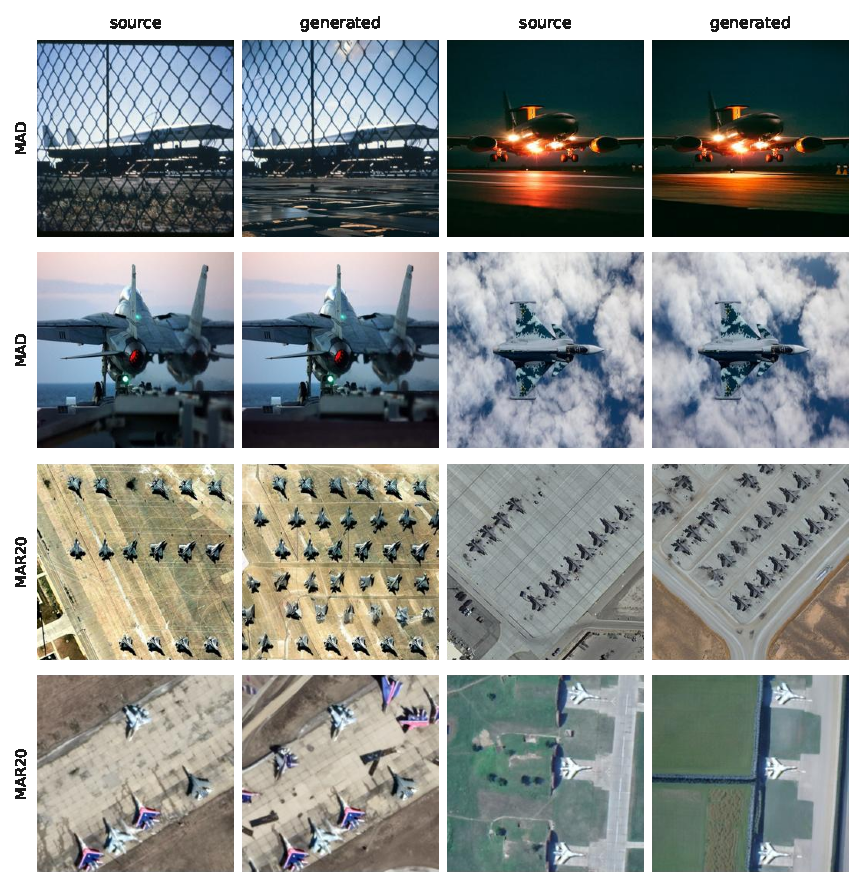
\includegraphics[width=0.92\linewidth]{figures/figa1_gallery.pdf}
\caption{Additional source/generated pairs (backgrounds regenerated;
all annotated objects protected). Top three rows: MAD; bottom row and
right half of row three: MAR20.}
\label{fig:gallery}
\end{figure}

\section{Per-class results}\label{app:perclass}
\begin{table}[h]\centering\small\caption{MAD tail classes: baseline test \mapm{} and per-arm $\Delta$ (3-seed means).}\label{tab:pc-mad-tail}
\begin{tabular}{lrrrrrrr}\toprule
Class & $n$ & base & tail-unif. & tail-prio. & weak-unif. & weak-prio. & RFS \\ \midrule
YF23 & 97 & 0.801 & -0.014 & +0.001 & -0.022 & -0.004 & +0.040 \\
AG600 & 153 & 0.763 & +0.059 & +0.032 & +0.041 & +0.018 & +0.034 \\
Be200 & 209 & 0.757 & +0.020 & +0.012 & +0.023 & -0.003 & +0.078 \\
P3 & 118 & 0.712 & -0.000 & +0.051 & +0.000 & +0.004 & +0.063 \\
XB70 & 119 & 0.656 & +0.041 & +0.077 & +0.055 & +0.014 & +0.103 \\
Mig31 & 225 & 0.636 & +0.101 & +0.101 & -0.006 & -0.010 & +0.132 \\
SR71 & 206 & 0.627 & +0.068 & +0.054 & +0.040 & +0.046 & +0.131 \\
Tu160 & 192 & 0.598 & +0.056 & +0.125 & +0.055 & +0.060 & +0.163 \\
E7 & 86 & 0.592 & +0.060 & +0.065 & +0.001 & +0.036 & +0.045 \\
Su34 & 210 & 0.565 & +0.072 & +0.058 & +0.030 & +0.075 & +0.045 \\
Tu95 & 197 & 0.505 & +0.169 & +0.132 & -0.042 & +0.110 & +0.144 \\
U2 & 208 & 0.439 & +0.084 & +0.088 & -0.015 & +0.009 & +0.106 \\
RQ4 & 212 & 0.404 & +0.062 & +0.010 & +0.027 & +0.030 & +0.194 \\
\bottomrule\end{tabular}\end{table}
\begin{table}[h]\centering\small\caption{MAD weak classes: baseline test \mapm{} and per-arm $\Delta$ (3-seed means).}\label{tab:pc-mad-weak}
\begin{tabular}{lrrrrrrr}\toprule
Class & $n$ & base & tail-unif. & tail-prio. & weak-unif. & weak-prio. & RFS \\ \midrule
Tornado & 273 & 0.561 & +0.047 & +0.048 & +0.123 & +0.096 & +0.106 \\
F4 & 411 & 0.555 & -0.026 & -0.036 & +0.014 & -0.015 & +0.052 \\
F35 & 746 & 0.518 & +0.029 & +0.035 & +0.046 & +0.076 & +0.066 \\
Mirage2000 & 297 & 0.513 & +0.041 & +0.039 & +0.069 & +0.056 & +0.183 \\
F15 & 851 & 0.481 & +0.014 & +0.032 & +0.030 & +0.023 & +0.106 \\
EF2000 & 388 & 0.475 & +0.053 & -0.015 & +0.059 & +0.048 & +0.158 \\
F16 & 902 & 0.468 & +0.048 & +0.028 & +0.070 & +0.046 & +0.095 \\
C17 & 348 & 0.465 & +0.013 & +0.026 & +0.060 & +0.068 & +0.148 \\
F22 & 450 & 0.450 & +0.032 & -0.004 & -0.011 & -0.018 & +0.004 \\
JAS39 & 350 & 0.428 & +0.018 & +0.013 & +0.010 & +0.024 & +0.193 \\
F18 & 885 & 0.416 & +0.022 & +0.013 & +0.042 & +0.024 & +0.091 \\
F14 & 358 & 0.331 & +0.030 & -0.129 & -0.006 & -0.040 & +0.177 \\
Rafale & 369 & 0.269 & +0.078 & +0.039 & +0.086 & +0.048 & +0.137 \\
\bottomrule\end{tabular}\end{table}
\begin{table}[h]\centering\small\caption{MAR20 (all 20 classes): baseline test \mapm{} and per-arm $\Delta$ (3-seed means).}\label{tab:pc-mar20}
\begin{tabular}{lrrrrrrr}\toprule
Class & $n$ & base & tail-unif. & tail-prio. & weak-unif. & weak-prio. & RFS \\ \midrule
A7 & 150 & 0.743 & +0.022 & +0.015 & +0.023 & -0.007 & -0.008 \\
A17 & 360 & 0.738 & -0.008 & +0.005 & -0.017 & -0.017 & +0.005 \\
A10 & 305 & 0.686 & -0.005 & -0.003 & -0.015 & -0.013 & -0.016 \\
A2 & 590 & 0.678 & +0.002 & +0.000 & -0.022 & -0.018 & -0.005 \\
A6 & 84 & 0.673 & +0.016 & +0.028 & +0.011 & -0.002 & +0.029 \\
A8 & 289 & 0.658 & -0.015 & +0.006 & -0.035 & -0.041 & +0.008 \\
A9 & 418 & 0.652 & +0.000 & -0.002 & -0.029 & -0.031 & -0.019 \\
A14 & 536 & 0.647 & +0.003 & +0.012 & -0.011 & -0.007 & +0.004 \\
A4 & 149 & 0.627 & +0.058 & +0.066 & +0.034 & +0.038 & +0.057 \\
A3 & 252 & 0.617 & +0.038 & +0.030 & +0.004 & -0.003 & +0.029 \\
A1 & 441 & 0.605 & -0.046 & -0.062 & -0.014 & -0.017 & -0.017 \\
A12 & 198 & 0.603 & -0.021 & -0.027 & +0.005 & +0.009 & -0.001 \\
A20 & 350 & 0.558 & -0.008 & -0.018 & +0.014 & +0.015 & +0.009 \\
A16 & 648 & 0.524 & +0.047 & +0.057 & +0.074 & +0.077 & -0.010 \\
A11 & 127 & 0.517 & -0.006 & +0.030 & -0.017 & -0.032 & -0.015 \\
A19 & 394 & 0.512 & +0.008 & -0.016 & +0.022 & +0.016 & -0.003 \\
A13 & 463 & 0.426 & +0.005 & -0.016 & +0.008 & +0.016 & +0.006 \\
A18 & 117 & 0.419 & +0.011 & +0.049 & -0.045 & -0.048 & +0.044 \\
A5 & 366 & 0.343 & +0.014 & +0.021 & +0.049 & +0.045 & -0.022 \\
A15 & 165 & 0.214 & +0.079 & +0.072 & +0.044 & +0.073 & -0.011 \\
\bottomrule\end{tabular}\end{table}
\section{Generation quality, hallucination audit, and object-level gate}\label{app:audit}
\paragraph{Quality metrics}
FID (torchmetrics FrechetInceptionDistance, Inception-V3 features) is computed per pool against the real training images containing that pool's target classes, so the reference sets differ across pools and cross-pool FID is indicative rather than strictly comparable; CLIPScore (\texttt{openai/clip-vit-base-patch16}) measures image--prompt similarity and LPIPS (AlexNet backbone) measures source--output distance, both on 200 sampled images per pool. The metrics were computed in the exploratory phase and therefore cover the three originally generated pools; the weak-uniform pool, generated later in the confirmatory phase, passed the same rule-based verification but was not scored.
\begin{table}[h]\centering\small\caption{Per-pool quality metrics (three exploratory-phase MAD pools).}\label{tab:quality}
\begin{tabular}{lrrrr}\toprule
Pool & FID & FID ref.\ ($n$ real) & CLIPScore & LPIPS \\ \midrule
tail-uniform & 89.7 & 1,797 & 19.6 $\pm$ 3.3 & 0.262 \\
tail-priority & 87.7 & 1,797 & 19.1 $\pm$ 3.8 & 0.244 \\
weak-priority & 100.4 & 3,744 & 20.2 $\pm$ 3.4 & 0.272 \\
\bottomrule\end{tabular}\end{table}
A detector-based scan of all 3{,}000 MAD synthetic images (the three originally generated pools) flagged images containing hallucinated, unlabeled aircraft. Table~\ref{tab:gate} reports per-pool removal statistics; a detector-based paired audit of a 450-image sample (150 per pool) flagged a net increase in off-mask detections in 10.2\% of images, consistent with the 11.1\% full-scan removal rate.
\begin{table}[h]\centering\small\caption{Object-level gate: full-corpus scan of the MAD pools.}\label{tab:gate}
\begin{tabular}{lrrrr}\toprule
Pool & images & removed & removed (\%) & flagged objects removed \\ \midrule
tail-priority & 1000 & 82 & 8.2 & 159 \\
tail-uniform & 1000 & 85 & 8.5 & 170 \\
weak-priority & 1000 & 165 & 16.5 & 516 \\
\midrule total & 3000 & 332 & 11.1 & 845 \\
\bottomrule\end{tabular}\end{table}
Retraining the three arms on gated pools (seed matched to the ungated runs) changed macro \mapm{} only marginally:
\begin{table}[h]\centering\small\caption{Gated $-$ ungated macro \mapm{} (single matched seed).}\label{tab:gated}
\begin{tabular}{lrrr}\toprule Arm & all & tail & weak \\ \midrule
tail-uniform & +0.005 & +0.009 & -0.009 \\
tail-priority & -0.017 & -0.012 & -0.021 \\
weak-priority & -0.001 & -0.002 & -0.008 \\
\bottomrule\end{tabular}\end{table}

\begin{figure}[h]\centering
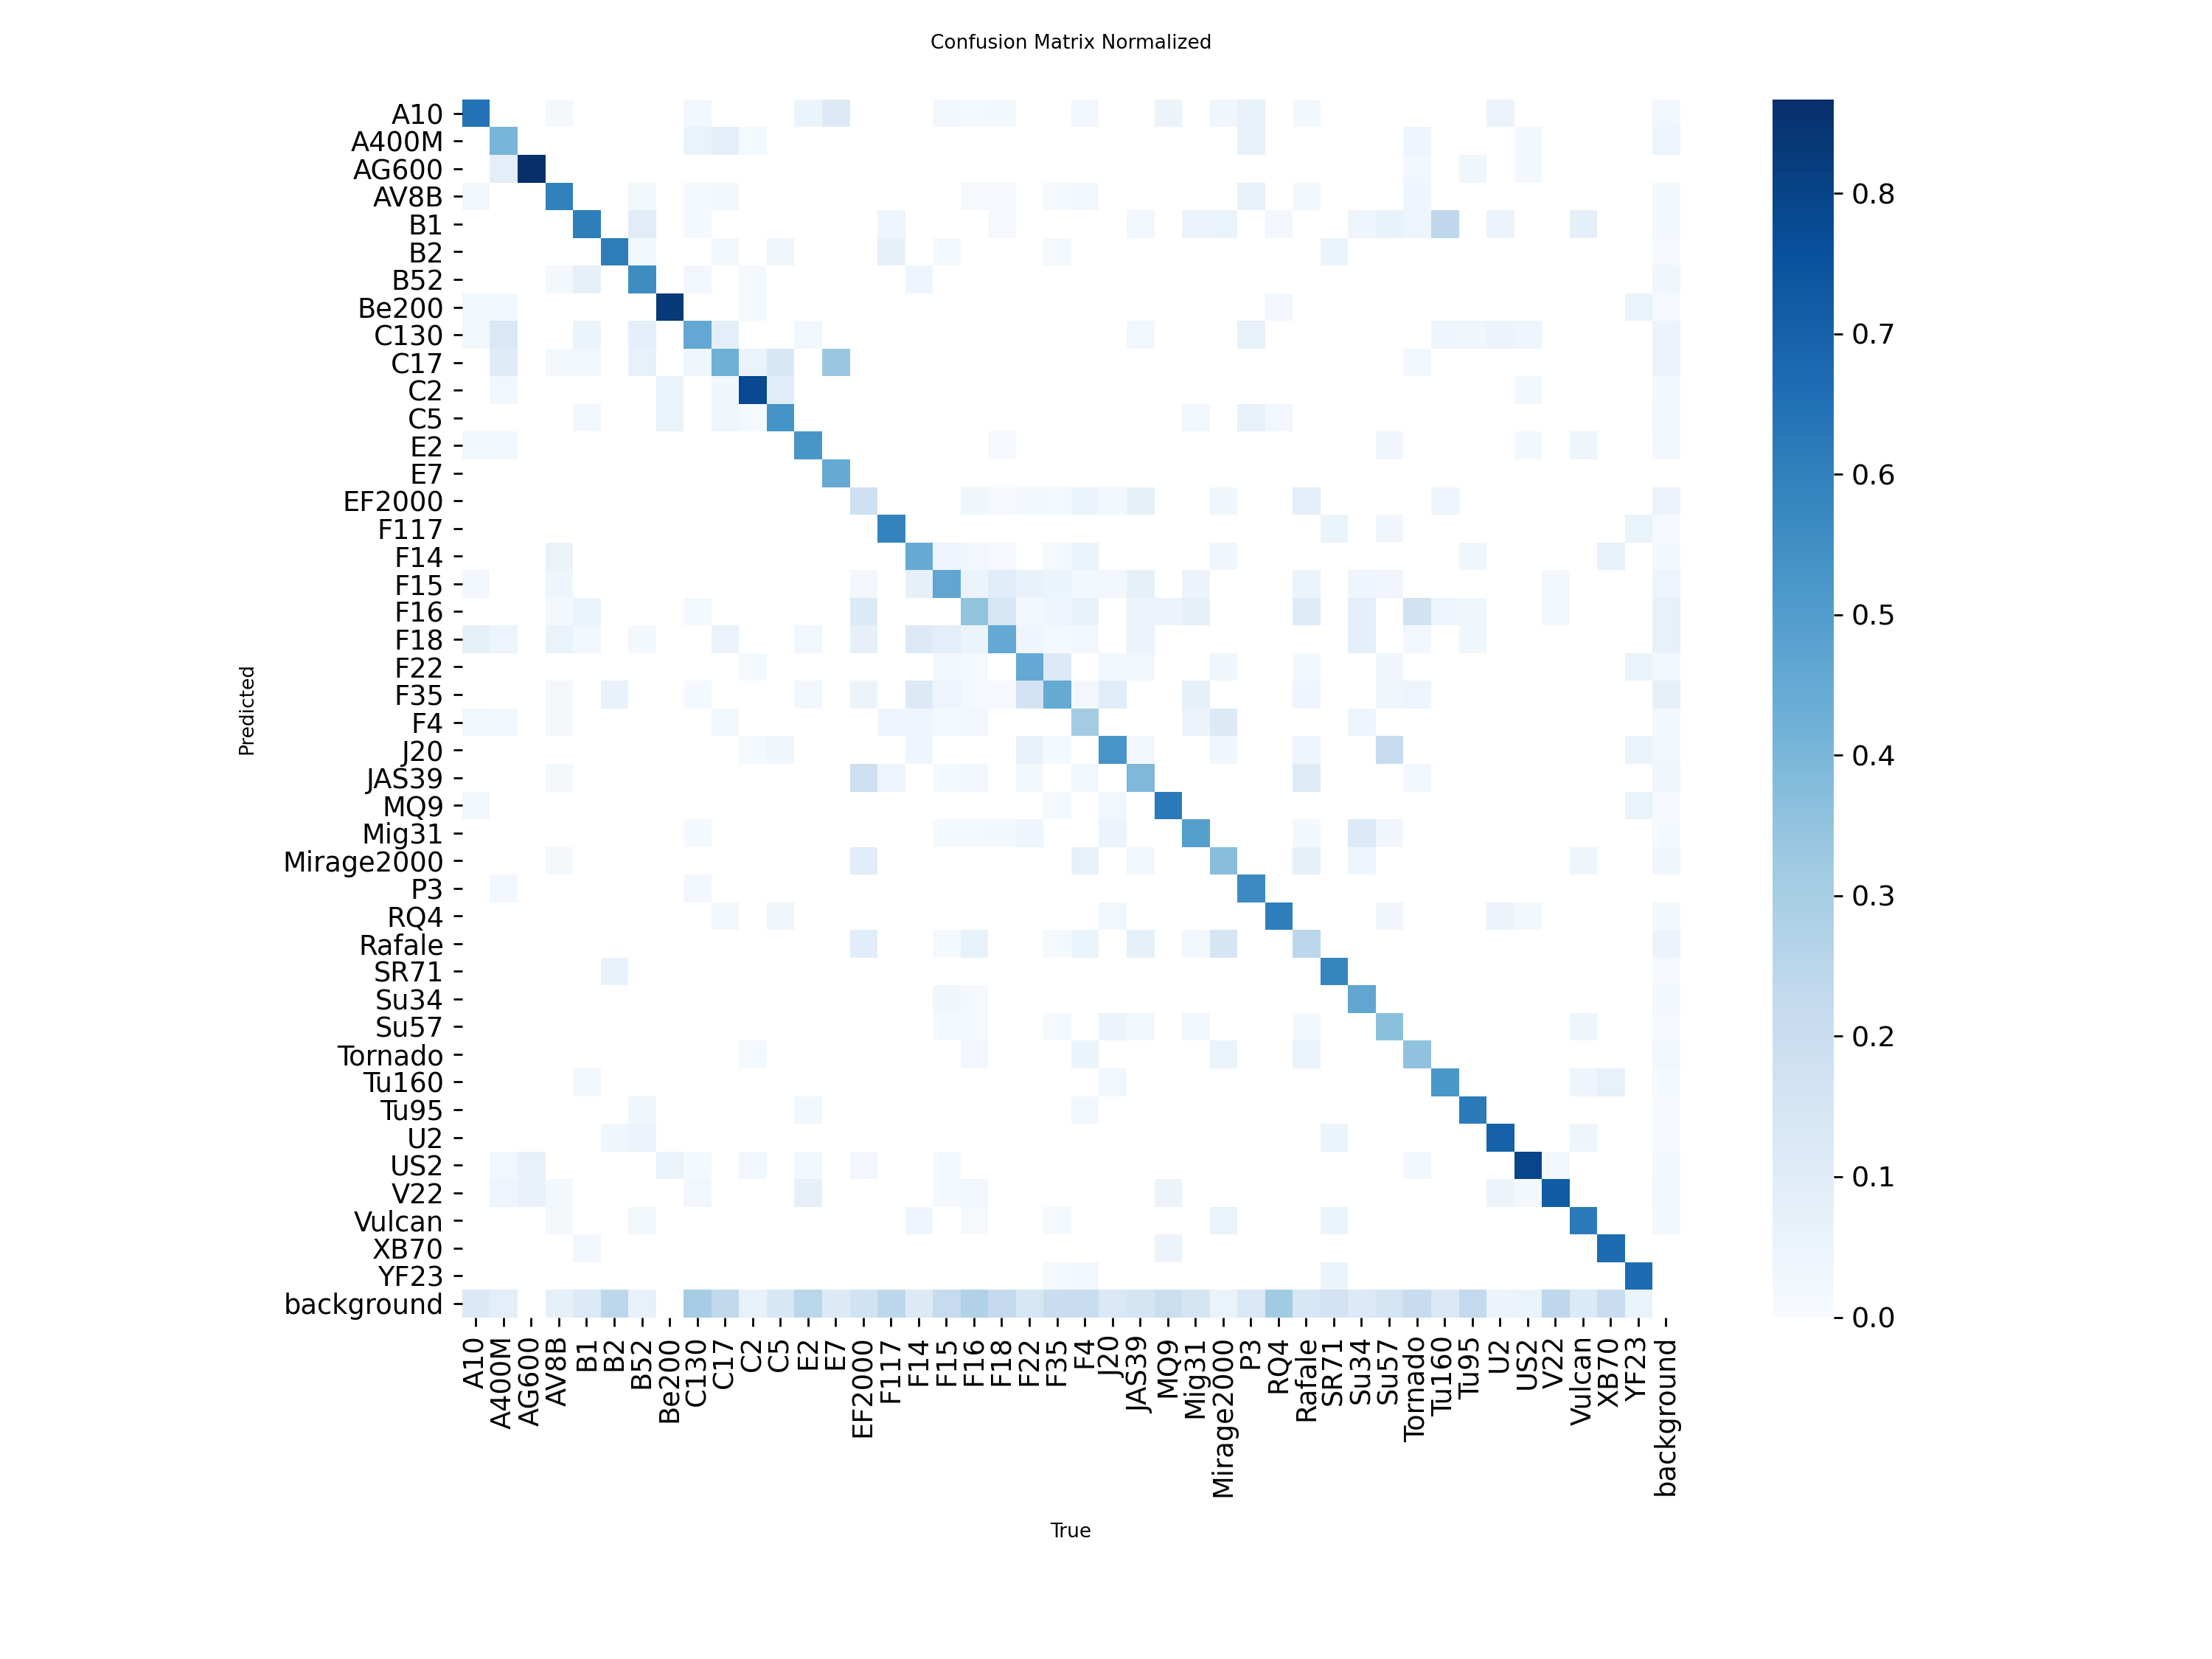
\includegraphics[width=0.9\linewidth]{figures/figa2_confusion.png}
\caption{Normalized confusion matrix of the MAD \texttt{basic\_aug}
baseline (one seed). The dominant off-diagonal mass lies in the
background row (missed detections), the error mode hypothesized to be
affected by background diversification (Section~\ref{sec:mechanism}).}
\label{fig:confusion}
\end{figure}

